\documentclass[conference]{IEEEtran}
\IEEEoverridecommandlockouts
\usepackage{cite}
\usepackage{amsmath,amssymb}
\usepackage{graphicx}
\usepackage{array}
\usepackage{url}
\usepackage[T1]{fontenc}

% Figures from the project's data; regenerate with: python paper/build.py
% Generated by paper/build.py from the project's data files. Do not edit.
\newcommand{\nInjAdv}{775}
\newcommand{\nInjAdvWithFix}{468}
\newcommand{\nReposUsable}{243}
\newcommand{\nOsvDate}{27 September 2026}
\newcommand{\nSeedSelected}{12}
\newcommand{\nSeedReserve}{4}
\newcommand{\nAdvSelected}{40}
\newcommand{\nAdvSelectedLinked}{34}
\newcommand{\nReviewItems}{40}
\newcommand{\nReviewConfirmed}{30}
\newcommand{\nReviewContested}{4}
\newcommand{\nReviewNeedsHuman}{4}
\newcommand{\nReviewRejected}{1}
\newcommand{\nReviewNotRecovered}{1}
\newcommand{\nCorrected}{4}
\newcommand{\nRecovered}{4}
\newcommand{\nCandidatePairs}{35}
\newcommand{\nEvents}{34}
\newcommand{\nEventsSound}{31}
\newcommand{\nEventsExcluded}{2}
\newcommand{\nEventsPending}{1}
\newcommand{\nEventsCross}{25}
\newcommand{\nEventsLocal}{6}
\newcommand{\nEventsSignedOff}{0}
\newcommand{\nSnapshotDate}{4 October 2026}
\newcommand{\nTests}{247}
\newcommand{\nRepoRows}{gitpython-developers/gitpython & BSD-3-Clause & 12 \\ \hline
parisneo/lollms\_legacy & Apache-2.0 & 9 \\ \hline
zauberzeug/nicegui & MIT & 4 \\ \hline
datadog/guarddog & Apache-2.0 & 3 (excluded: size) \\ \hline
ietf-tools/xml2rfc & BSD-3-Clause & 3 \\ \hline
mar10/wsgidav & MIT & 2 \\ \hline
sqlalchemy/mako & MIT & 2 \\ \hline
alerta/alerta & Apache-2.0 & 1 \\ \hline
collerek/ormar & MIT & 1 \\ \hline
geopython/pycsw & MIT & 1 \\ \hline
piccolo-orm/piccolo & MIT & 1 \\ \hline
tortoise/tortoise-orm & Apache-2.0 & 1 \\ \hline}


\begin{document}

% Generated by paper/build.py. Edit META in build.py, not this file.
\title{GraphGate: Toward an In-Loop Security Gate for Iterative LLM Code Refinement Using Temporal Code-Graph Deltas}

\author{\IEEEauthorblockN{Janani R}
\IEEEauthorblockA{Department of Artificial Intelligence and Data Science \\
Karunya Institute of Technology and Sciences \\
Coimbatore, India \\
email address}
\and
\IEEEauthorblockN{Rajkumar}
\IEEEauthorblockA{Project Guide, Department of Artificial Intelligence and Data Science \\
Karunya Institute of Technology and Sciences \\
Coimbatore, India \\
email address}}

\maketitle

\begin{abstract}
Developers rarely accept the first answer a code assistant gives them; they ask a large language model (LLM) for one revision after another. A recent controlled study found that critical vulnerabilities grew by 37.6\% after only five such rounds~\cite{shukla2025degradation}. Checks that inspect only the changed lines miss many of these regressions, because the vulnerable data flow often starts or ends in a file the revision never touched. We present GraphGate, a security gate that sits inside the refinement loop, compares the code graphs of consecutive revisions and applies four deterministic rules to their difference, using an LLM only to triage and explain what the rules flag. This paper reports the design and the first milestone: a refinement harness whose traces replay byte for byte, the evidence behind our choice of code-generation model, and a benchmark built from real injection-class fixes. From \nInjAdv{} Python security advisories we selected \nSeedSelected{} permissively licensed projects, verified every fix link with two independent reviewers, and extracted \nEvents{} candidate regression events labelled local or cross-file by a pre-registered rule. We close with the protocol that will compare no gate, a diff-only gate and GraphGate on identical replayed traces.
\end{abstract}

\begin{IEEEkeywords}
large language models, secure code generation, iterative refinement, taint analysis, code property graphs
\end{IEEEkeywords}

\section{Introduction}
\label{sec:intro}

AI coding assistants are used conversationally. A developer asks for a function, reads it, and then asks again: make it faster, add a feature, tidy it up. Most of what we know about the security of generated code, however, comes from judging single responses~\cite{pearce2022asleep,perry2023insecure,khoury2023secure}. Shukla et al.~\cite{shukla2025degradation} studied the loop itself: across 400 code samples and 40 rounds of requested improvements, security got worse as the rounds went on. They deliberately left out any intervention and named verification inside the loop as the follow-up that was needed.

The obvious intervention is to check each revision before accepting it, but practical checks are local to the change: a pattern scanner such as Semgrep~\cite{semgrep} or Bandit~\cite{bandit} run on the diff, or an LLM reviewer shown the changed lines. Many injection flaws are not local. A revision can weaken a validation helper that other modules rely on, change a default so that a distant call becomes unsafe, or open a call path that routes user input around an existing guard. The diff can then look harmless, because the danger lies in code the diff does not show.

GraphGate represents each revision as a code graph of symbols, calls, taint edges and sanitizers, and reasons about the \emph{difference} between the graphs of consecutive revisions. Four deterministic rules look for sanitizer removal, new source-to-sink paths, eliminated guards and shortened paths, and an LLM then classifies each flag and writes a rationale that can be fed into the next prompt. Keeping detection in deterministic rules makes it testable, and keeping the LLM in a triage role limits the room it has to invent findings.

Our research question is whether this cross-file grounding reduces security degradation compared with no gate and with a gate restricted to the diff. Answering it needs a harness whose runs can be replayed exactly, a benchmark of real regressions with trustworthy labels, and a protocol fixed in advance. This paper contributes:
\begin{itemize}
\item a gate design based on temporal code-graph differencing, with a deliberately narrow role for the LLM (Section~\ref{sec:design});
\item a refinement harness with byte-identical replay, the models used and the evidence for choosing them (Section~\ref{sec:infra});
\item a benchmark pipeline with independent verification of every fix link and a pre-registered local/cross-file rule (Section~\ref{sec:dataset});
\item a pre-registered evaluation protocol (Section~\ref{sec:eval}).
\end{itemize}
The graph builder and difference rules are designed but not yet implemented, so no detection results are reported; the numbers here describe the parts that are finished.

\section{Related Work}
\label{sec:related}

\textit{Security of generated code.} Pearce et al.~\cite{pearce2022asleep} found that roughly 40\% of programs GitHub Copilot produced for scenarios built on MITRE's dangerous weaknesses~\cite{mitrecwe} were vulnerable. In a user study by Perry et al.~\cite{perry2023insecure}, participants with an AI assistant wrote less secure code while feeling more confident about it, and Khoury et al.~\cite{khoury2023secure} judged only five of 21 ChatGPT programs secure on the first attempt. These studies evaluate single responses. Iteration is usually presented as a way to improve output~\cite{madaan2023selfrefine}, although the gains of self-repair for code are modest and bounded by the quality of the feedback~\cite{olausson2024selfrepair}; Shukla et al.~\cite{shukla2025degradation} showed that it can also erode security, with distinct vulnerability patterns for different prompting strategies.

\textit{Static analysis and code graphs.} Taint analysis reports flows of untrusted data that reach a sensitive sink without passing a sanitizer~\cite{livshits2005finding}, and FlowDroid~\cite{arzt2014flowdroid} showed how precise it can be. Yamaguchi et al.~\cite{yamaguchi2014cpg} merged syntax trees, control flow and program dependences into a queryable code property graph, an idea implemented in the Joern platform~\cite{joern}. For Python, Pysa~\cite{pysa} performs taint analysis on top of the Pyre type checker, and CodeQL~\cite{codeql} offers data-flow queries. These tools analyse snapshots; they can be rerun after every revision, and we use them as baselines, but they do not reason about what changed or explain findings in a form that can steer the next step.

\textit{Learning-based and LLM-based detection.} Early detectors trained graph neural networks or transformers on labelled functions~\cite{zhou2019devign,fu2022linevul}, but much of their reported accuracy does not survive realistic evaluation, partly because datasets contain label noise and duplicates~\cite{ding2025primevul}. Recent systems pair LLMs with program analysis: IRIS~\cite{li2025iris} infers taint specifications for a static analyser, LLMDFA~\cite{wang2024llmdfa} performs data-flow analysis with an LLM, LLMxCPG~\cite{lekssays2025llmxcpg} gives an LLM compact graph slices and cuts the code it must read by 67.84--90.93\%, RepoAudit~\cite{guo2025repoaudit} explores whole repositories with an agent, and MulVul~\cite{wu2026mulvul} routes code to specialised detector agents. All of them look at code at one point in time.

\textit{Benchmarks and reproducibility.} Big-Vul~\cite{fan2020bigvul} and CVEfixes~\cite{bhandari2021cvefixes} pair vulnerabilities with fixing commits, but automatically collected links can be wrong~\cite{ding2025primevul}; we take advisories from OSV~\cite{osv}, which aggregates the GitHub Advisory Database~\cite{ghadvisory}, and verify every link. LLM code generation is non-deterministic even at temperature zero~\cite{ouyang2025nondeterminism}, and closed models that change over time threaten reproducibility~\cite{sallou2024breaking}; our design therefore relies on replayed traces. Table~\ref{tab:related} summarises the gap: no prior work evaluates a graph-grounded gate inside the refinement loop or reasons over the difference between successive versions.

\begin{table}[t]
\caption{Position of GraphGate relative to prior work}
\label{tab:related}
\centering
\footnotesize
\begin{tabular}{|p{1.9cm}|p{1.8cm}|p{1.7cm}|p{1.2cm}|}
\hline
\textbf{Work} & \textbf{Setting} & \textbf{Context used} & \textbf{Across revisions} \\
\hline
Shukla et al.~\cite{shukla2025degradation} & Iterative refinement & None (measurement) & Measures only \\
\hline
Pysa, CodeQL~\cite{pysa,codeql} & Static taint analysis & Whole program & No \\
\hline
LLMxCPG~\cite{lekssays2025llmxcpg} & LLM with graph slices & CPG slice & No \\
\hline
IRIS, RepoAudit~\cite{li2025iris,guo2025repoaudit} & LLM with analysis or agent & Repository & No \\
\hline
GraphGate (ours) & In-loop gate & Graph delta around changes & Yes \\
\hline
\end{tabular}
\end{table}

\section{GraphGate Design}
\label{sec:design}

\subsection{Research Questions}
The project is organised around four questions. \textbf{RQ1:} does a graph-differencing gate reduce security degradation across refinement iterations, compared with no gate and with an otherwise identical diff-only gate? \textbf{RQ2:} what is its recall on cross-file regressions, and how many iterations pass before one is caught? \textbf{RQ3:} does it outperform mature static taint analysers used alone? \textbf{RQ4:} what does it cost in false alarms, latency and tokens, and which graph components matter?

\subsection{Overview and Deployment}
Fig.~\ref{fig:arch} shows the gate. Before a candidate revision is accepted, it runs Semgrep and Bandit on the diff, then the graph-difference engine, then LLM triage of whatever was flagged. A blocked revision is not committed and its rationale joins the next prompt; an allowed revision is committed and its files are re-indexed into the graph. The targets are a pre-merge check in continuous integration and middleware in an agent framework, for example a LangGraph~\cite{langgraph} node between the generation and commit steps. Both tolerate a few seconds of added latency; interactive editor use, with its tighter budget, is out of scope.

\begin{figure}[t]
\centering
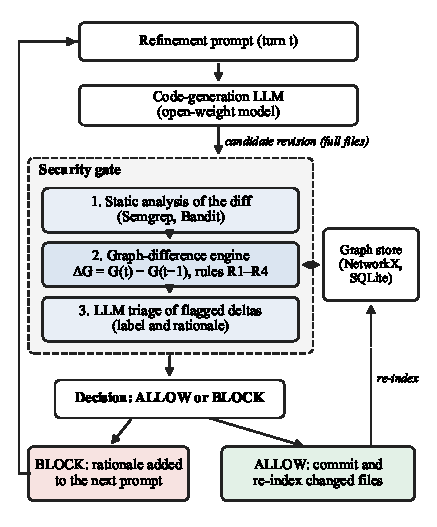
\includegraphics[width=0.86\columnwidth]{figures/architecture}
\caption{GraphGate inside the refinement loop. The LLM only triages what the deterministic stages flag.}
\label{fig:arch}
\end{figure}

\subsection{Code Graph}
The graph of revision $t$ is $G(t) = (V, E_{\mathrm{call}}, E_{\mathrm{taint}}, E_{\mathrm{sanitize}})$. Vertices are function, method and module symbols from tree-sitter~\cite{treesitter} syntax trees. Call edges are resolved only for calls within a module, calls through static imports and attribute calls whose receiver class is statically known; any other call becomes an explicit \emph{unknown} edge, so the analysis can report what it could not see. Taint edges link sources (request parameters, environment variables, file and network input, command-line arguments) to uses through assignments and call arguments, flow-insensitively across procedures. Sanitizers are symbols matching an allowlist seeded from Semgrep and Pysa rules. Graphs are held in NetworkX~\cite{hagberg2008networkx} and persisted between iterations.

\subsection{Difference Rules and Triage}
After each revision the engine computes $\Delta G = G(t) - G(t-1)$ within two hops of the changed symbols; the depth is an ablation variable. Four rules are applied to the difference.
\begin{itemize}
\item \textbf{R1, sanitizer removal:} a sanitizer present before is absent or bypassed while its callers remain.
\item \textbf{R2, new path:} a source-to-sink path exists that did not exist before.
\item \textbf{R3, guard elimination:} a guard on an existing source-to-sink path disappears.
\item \textbf{R4, path shortening:} the shortest sanitizer-free path from a source to a sink gets shorter.
\end{itemize}
Each rule is a pure function of two graphs and is unit-tested on hand-built graphs before it runs on real code. The triage LLM receives each flag with its supporting subgraph and labels it an exploitable regression, a benign refactor or uncertain. It is never asked to search the code on its own, which keeps the detector testable and narrows the room for invented findings.

The scope is Python and the injection family: SQL injection (CWE-89), OS command injection (CWE-78), command injection in general (CWE-77) and path traversal (CWE-22)~\cite{mitrecwe}. The graph does not model monkey-patching, reflection or framework-generated routing, so results will describe practical, lightweight differencing rather than a sound analysis, and unknown-edge counts will be reported per repository.

\section{Experimental Infrastructure}
\label{sec:infra}

\subsection{Refinement Harness}
The harness drives a refinement loop over a set of Python files. Each turn sends the model a fixed system prompt, every current file and one instruction; the model returns complete files, and the harness computes a diff and appends a record to a JSON Lines trace holding the prompt and its hash, the requested and the served model identifiers, the parameters, the response, token usage, latency and the diff. Refusals and errors have their own record kinds. Each prompt sequence is run several times, and every run carries a replication number. The code is Python 3.12 with pinned dependencies and \nTests{} automated tests.

\subsection{Reproducibility Without Sampling Controls}
The original plan specified a temperature of zero and fixed seeds, but current Anthropic models reject sampling parameters and the API has never accepted a seed; a zero temperature would not have guaranteed identical output anyway~\cite{ouyang2025nondeterminism}. Reproducibility therefore rests on a response cache keyed by (prompt hash, replication) and on replay: the gate conditions never call the model but consume recorded traces, so every condition sees the same revisions. Traces recorded against the live API replay byte for byte.

Two pitfalls are worth reporting because they fail silently. Our first cache used the prompt hash alone as its key; because the API takes no seed, all replications send identical requests, so the cache served the first replication's answer to the others and \emph{N} replications collapsed into one. Statistical tests would still have run, over duplicates. Adding the replication number to the key fixed this, and a regression test guards it. Second, the API reports a dated snapshot name (for example \texttt{claude-haiku-4-5-20251001}) that differs from the name requested, which broke the hash check on replay; the harness now records both.

\subsection{Models Used}
Table~\ref{tab:models} lists the models~\cite{anthropicmodels}. The newest models declined part of the workload on a harmless fixture (a small user-lookup module that already used parameterised queries, refined with three instructions in the style of the base study), and a declined turn ends its replication. We therefore use \texttt{claude-opus-4-8}, which completed all 18 turns, with adaptive thinking, medium effort and at most 16,000 output tokens per turn. The smaller \texttt{claude-haiku-4-5} serves the planned small-model ablation. Model identifiers are command-line options and every trace records them. A refusal is stored as an outcome with its category, is never cached and never triggers a fallback to another model, which would mix models within a condition. Because refusals are likely to rise on genuinely vulnerable code, the refusal rate will be reported beside the degradation curve.

\begin{table}[t]
\caption{Models used and smoke-run results on a harmless fixture}
\label{tab:models}
\centering
\footnotesize
\begin{tabular}{|p{2.05cm}|p{2.55cm}|p{2.6cm}|}
\hline
\textbf{Model} & \textbf{Role} & \textbf{Smoke runs (3 prompts)} \\
\hline
claude-opus-4-8 & Code generation (primary) & 18 of 18 turns, no refusals \\
\hline
claude-haiku-4-5 & Small-model ablation & 18 of 18 turns, no refusals \\
\hline
claude-opus-5-5 & Evaluated, not used & 2 of 7 turns refused \\
\hline
claude-opus-5 & Evaluated, not used & Refused in every run \\
\hline
claude-opus-5-5 agents (Claude Code) & Dataset curation assistance & Every label needs author sign-off \\
\hline
\end{tabular}
\end{table}

\section{Benchmark Construction}
\label{sec:dataset}

Each event is a real fix, inverted: the fixed code is the clean state and the vulnerable code is the regression that will be injected into a refinement trace. The targets are 25 to 30 validated events for the first milestone and 40 to 60, a third or more of them cross-file, for the full study. Table~\ref{tab:funnel} and Fig.~\ref{fig:funnel} trace the pipeline.

\subsection{Advisories and Seed Repositories}
From the OSV export for PyPI~\cite{osv}, retrieved on \nOsvDate{} and pinned by its hash, we kept reviewed GitHub advisories (only these carry CWE identifiers) with an injection CWE, giving \nInjAdv{} advisories, \nInjAdvWithFix{} of them linking a fix, across \nReposUsable{} repositories. Seed repositories must be MIT, Apache-2.0 or BSD licensed, so that traces can be redistributed, and hold 5,000 to 50,000 lines of Python outside tests and documentation. We selected \nSeedSelected{} (Table~\ref{tab:repos}) and kept \nSeedReserve{} in reserve. Path traversal dominates, so results will be reported per class.

\begin{table}[t]
\caption{Selected seed repositories}
\label{tab:repos}
\centering
\footnotesize
\begin{tabular}{|p{3.3cm}|p{1.6cm}|p{1.9cm}|}
\hline
\textbf{Repository} & \textbf{Licence} & \textbf{Advisories} \\
\hline
\nRepoRows
\end{tabular}
\end{table}

\subsection{Fix Pairs and Their Verification}
The resolver takes the earliest linked commit on the default branch as the fix and its first parent as the vulnerable version, and re-measures size and licence at that commit; this removed one repository whose code was only 1,200 to 4,200 lines at every vulnerable commit. Two independent reviewers then checked each pair, one asked to establish the link and one to refute it, and advisories without a linked fix got a history search. Of \nReviewItems{} items, \nReviewConfirmed{} were confirmed outright. Reading every other case against the history, we corrected \nCorrected{} pairs where both reviewers named the same other commit (one advisory also linked the commit that \emph{introduced} the bug, one linked only backports, two described multi-part fixes) and recovered \nRecovered{} missing fixes. The simple linking rule was thus wrong for about one advisory in eight. Corrections and recoveries are kept in separate files so that every commit not taken from an advisory can be audited.

\begin{table}[t]
\caption{From advisories to regression events}
\label{tab:funnel}
\centering
\footnotesize
\begin{tabular}{|p{5.2cm}|p{1.6cm}|}
\hline
\textbf{Stage} & \textbf{Count} \\
\hline
Injection-class PyPI advisories (reviewed, not withdrawn) & \nInjAdv \\
\hline
... with at least one linked fix commit & \nInjAdvWithFix \\
\hline
Advisories in the selected seed repositories & \nAdvSelected \\
\hline
Candidate vulnerable/fixed pairs after verification & \nCandidatePairs \\
\hline
Candidate events (shared fixes merged) & \nEvents \\
\hline
Prepared and passed the adversarial check & \nEventsSound \\
\hline
Excluded during preparation & \nEventsExcluded \\
\hline
Still in preparation (\nSnapshotDate) & \nEventsPending \\
\hline
\end{tabular}
\end{table}

\begin{figure}[t]
\centering
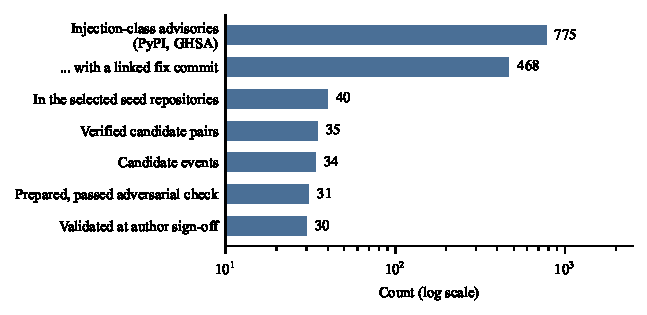
\includegraphics[width=\columnwidth]{figures/funnel}
\caption{Dataset funnel, from advisories to prepared events.}
\label{fig:funnel}
\end{figure}

\subsection{Extracting Events}
The model rewrites whole files, and 16 of the 35 candidate pairs have a file on the vulnerable flow of more than about 14,000 tokens. Each event is therefore a \emph{trimmed slice}: the files on the flow at their real paths, cut down to the functions between the entry point, the guard the fix added and the sink. A clean version is cut at the fix commit and a regressed version at the vulnerable commit. The slicer keeps source text verbatim and reports every referenced name it removed, and comments that describe the vulnerability or the fix are stripped from both versions and logged, because the model sees every file verbatim.

An event is \emph{local} if entry, guard and sink lie in one file, and \emph{cross-file} otherwise; this rule was fixed before any event was built, and the label follows the real sink even when a large sink function is represented by its call site. For each event an LLM analyst builds the slice, an independent LLM checker tries to refute it, and only the authors' sign-off validates it. At the time of writing \nEventsSound{} events had passed the check, \nEventsCross{} of them cross-file (Fig.~\ref{fig:scope}), and \nEventsExcluded{} were excluded. One exclusion is a finding in itself: our analysis indicates that a published fix sanitises a document that the command-line PDF path then discards and re-parses, leaving that path vulnerable. The other reflected a limit of our own tooling: the slicer could not keep a module-level block that connects an upload handler to its sink. The slicer has since been extended to keep such wiring on request, and one event whose parser grammar is assembled at module level was rebuilt with it and awaits a second check. In every prepared event the checker independently arrived at the same class and the same scope label as the analyst.

\begin{figure}[t]
\centering
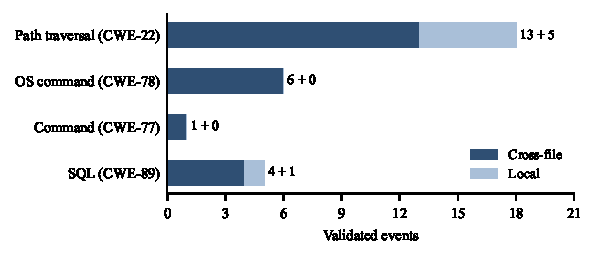
\includegraphics[width=\columnwidth]{figures/scope}
\caption{Prepared events by vulnerability class and scope.}
\label{fig:scope}
\end{figure}

\section{Evaluation Protocol}
\label{sec:eval}

\subsection{Traces, Conditions and Baselines}
Each validated event becomes a refinement trace of five to eight turns (improve readability, add a feature, optimise), with the regression injected at a random turn between the second and the sixth and every turn labelled clean, local regression or cross-file regression. Injected patterns that already occur elsewhere in the repository are excluded from the graph's retrieval scope to avoid leakage. All conditions in Table~\ref{tab:conditions} consume the same recorded traces, so only the gate's context and detector vary.

\begin{table}[t]
\caption{Gate conditions and baselines}
\label{tab:conditions}
\centering
\footnotesize
\begin{tabular}{|p{1.3cm}|p{3.4cm}|p{2.4cm}|}
\hline
\textbf{Condition} & \textbf{Configuration} & \textbf{Question} \\
\hline
A & No gate & Baseline degradation \\
\hline
B & Semgrep, Bandit and LLM triage on the diff & Conventional check \\
\hline
C, GraphGate & B plus the graph-difference engine & RQ1, RQ2 \\
\hline
S1, S2 & Pysa; CodeQL if licensing allows (no LLM) & RQ3 \\
\hline
\end{tabular}
\end{table}

\subsection{Metrics, Ablations and Success Criteria}
We will report the degradation curve, cross-file recall, iterations to detection, the false-positive burden (BLOCK decisions on clean turns), latency, tokens, cost and the refusal rate. Traces are replayed over several replications, and B against C and C against S1 are compared with paired Wilcoxon signed-rank tests~\cite{wilcoxon1945} on per-trace recall, with effect sizes. Ablations remove call or taint edges, vary the hop depth from one to three, drop LLM triage and swap in the smaller model.

The success criteria were fixed in advance: condition A reproduces the degradation trend of the base study, condition C improves cross-file recall over B significantly and is competitive with S1, and C keeps false positives below about 15\% of clean turns with a median added latency under about 10 seconds. A null result on the cross-file comparison would still be reported, because the controlled design is part of the contribution.

\section{Early Observations}
\label{sec:obs}

\textit{Frontier models may decline refinement work.} A loop built on such a model loses turns exactly where code is security-relevant, and dropping those turns would understate degradation; refusals must be reported as outcomes. \textit{Caching can erase replications,} as described in Section~\ref{sec:infra}, without any visible failure. \textit{Fix links need checking:} besides the corrected links, our analysis indicates that one published fix did not close the flow it targeted. \textit{A regression-like change already appeared} in a smoke run: asked to ``optimize the database access'', one replication of \texttt{claude-opus-4-8} interpolated a column name into SQL with an f-string. \textit{Scope depends on structure:} in GitPython every command runs through one central function, so its events are cross-file even when the visible change is inside one method, and results will be reported per repository.

\section{Threats to Validity}
\label{sec:threats}

\textit{Construct.} A regression is defined as an inverted real fix, and only the injection family is covered; the local/cross-file label follows one operational rule, which is why it was fixed before the events were built. \textit{Internal.} LLM non-determinism is controlled by replay. LLM agents assisted curation, so every such step has an adversarial check and author sign-off; stripped comments may still leave cues such as identifiers that mention unsafe options. \textit{External.} Injected regressions in synthetic traces may differ from natural ones, so a holdout of real multi-turn sessions, reviewed manually and never used for tuning, is planned. The dataset is dominated by path traversal and one library supplies about a third of the events. \textit{Conclusion.} The number of events is modest; paired non-parametric tests, effect sizes and oversampling of cross-file events keep conclusions conservative. Public advisories may also appear in model training data.

\section{Conclusion}
\label{sec:conclusion}

Iterative refinement with LLMs can erode security, and diff-only checks miss regressions whose data flow crosses file boundaries. GraphGate reasons over the difference between code graphs of successive revisions and limits the LLM to triage. We have presented its design, a harness with exact replay, the models used and why, and a verified benchmark pipeline with a pre-registered scope rule. Work continues in two milestones. The first completes the author sign-off of the prepared events, synthesises refinement traces from them, and runs the diff-only gate and Pysa over those traces to obtain an A-versus-B-versus-S1 degradation result, together with iterations to detection and false-positive figures; this is a reportable study on its own. The second builds the graph layer, implements rules R1 to R4 with their unit tests, adds cross-file variants to the dataset and runs condition C with its ablations, followed by evaluation on the real-session holdout. Traces, labels, rules and the harness will be released under a permissive licence once the licence check of every seed repository is complete.

\section*{Acknowledgment}
The authors thank the Karunya Institute of Technology and Sciences for its support. In line with IEEE policy, we disclose that Anthropic's Claude, through Claude Code, assisted with implementing the software, with the dataset verification in Section~\ref{sec:dataset}, and with drafting this manuscript; the authors reviewed all of it and take full responsibility for the content.

\bibliographystyle{IEEEtran}
\bibliography{references}

\end{document}
